%%%%%%%%%%%%%%%%%%%%%%%%%%%%%%%%%%%%%%%%%
% a0poster Portrait Poster
% LaTeX Template
% Version 1.0 (22/06/13)
%
% The a0poster class was created by:
% Gerlinde Kettl and Matthias Weiser (tex@kettl.de)
% 
% This template has been downloaded from:
% http://www.LaTeXTemplates.com
%
% License:
% CC BY-NC-SA 3.0 (http://creativecommons.org/licenses/by-nc-sa/3.0/)
%
%%%%%%%%%%%%%%%%%%%%%%%%%%%%%%%%%%%%%%%%%

%----------------------------------------------------------------------------------------
%	PACKAGES AND OTHER DOCUMENT CONFIGURATIONS
%----------------------------------------------------------------------------------------

\documentclass[a0,portrait]{a0poster}

\usepackage{multicol} % This is so we can have multiple columns of text side-by-side
\columnsep=100pt % This is the amount of white space between the columns in the poster
\columnseprule=3pt % This is the thickness of the black line between the columns in the poster

\usepackage[svgnames]{xcolor} % Specify colors by their 'svgnames', for a full list of all colors available see here: http://www.latextemplates.com/svgnames-colors

\usepackage{times} % Use the times font
%\usepackage{palatino} % Uncomment to use the Palatino font

\usepackage{graphicx} % Required for including images
\graphicspath{{figures/}} % Location of the graphics files
\usepackage{booktabs} % Top and bottom rules for table
\usepackage[font=small,labelfont=bf]{caption} % Required for specifying captions to tables and figures
\usepackage{amsfonts, amsmath, amsthm, amssymb} % For math fonts, symbols and environments
\usepackage{wrapfig} % Allows wrapping text around tables and figures
\usepackage{amsmath}
\usepackage{amssymb}
\usepackage{natbib}
\usepackage{graphicx}
\usepackage{url}
\usepackage{xfrac}
\usepackage{esvect}
\usepackage{varwidth} 
\usepackage{physics}
\usepackage{tensor}
\usepackage{microtype}
%%%%%%%%%%%%%Floating table solutions %%%%%%%%%%%%%%%%%%
\usepackage{float}
\restylefloat{table}

%%%%%%%%%%%%%%%%%%%%%%%%%%%%%%%%%%%%%%%%%
\newcommand{\driv}[2]{\frac{d #1}{d #2}}
\newcommand{\con}{\frac{8\pi}{3}G}
\newcommand{\brac}[1]{\left(#1\right)}
\newcommand{\bracc}[1]{\left[#1\right]}
%%%%%%%%%%%%%%%%%%%%%%%%%%%%%%%%%%%%%%%%%%
%%%%%LINESPACING%%%%%%%%%
\renewcommand{\baselinestretch}{0.85}
\usepackage{titlesec}




\titlespacing\section{3pt}{0pt plus 0pt minus 2pt}{0pt plus 0pt minus 2pt}
\titlespacing\subsection{3pt}{0pt plus 0pt minus 2pt}{0pt plus 0pt minus 2pt}
\titlespacing\subsubsection{0pt}{0pt plus 0pt minus 2pt}{0pt plus 0pt minus 2pt}

\begin{document}

%----------------------------------------------------------------------------------------
%	POSTER HEADER 
%----------------------------------------------------------------------------------------

% The header is divided into two boxes:
% The first is 75% wide and houses the title, subtitle, names, university/organization and contact information
% The second is 25% wide and houses a logo for your university/organization or a photo of you
% The widths of these boxes can be easily edited to accommodate your content as you see fit

\begin{minipage}[b]{0.75\linewidth}
\veryHuge \color{NavyBlue} \textbf{Solving the Friedman equation for a Dark Fluid equation of state.} \color{Black}\\ % Title
%\Huge\textit{An Exploration of Complexity}\\[2cm] % Subtitle
\huge \textbf{Pieter vd Merwe }\\[0.5cm] % Author(s)
\huge North-West University \\ Center for Space Research\\[0.4cm] % University/organization
\Large \texttt{25957937@nwu.ac.za}\\
\end{minipage}
%
\begin{minipage}[b]{0.25\linewidth}

\includegraphics[width=20cm]{nwu-logo.jpg}\\

\includegraphics[width=20cm]{NASSP_Logo.jpg}\\
\end{minipage}

\vspace{1cm} % A bit of extra whitespace between the header and poster content

%----------------------------------------------------------------------------------------

\begin{multicols}{2} % This is how many columns your poster will be broken into, a portrait poster is generally split into 2 columns

%----------------------------------------------------------------------------------------
%	ABSTRACT
%----------------------------------------------------------------------------------------

\color{Navy} % Navy color for the abstract

\begin{abstract}

Dark energy and dark matter account for nearly 95\% of the matter-energy content of the universe, yet very little is known about both dark energy and dark matter. We aim to look at the impact of unifying Dark energy and Dark matter into a single Dark fluid Equation of state and solving the Friedman equations for such a fluid. The first candidate that is looked at is the Chaplygin gas Equation of state. The behaviour of the expansion coefficient is looked at for different epochs. The Friedman equations are also solved for a pure dark fluid parametrization Equation of state and the behaviour of the accelerated expansion for this equation of state is investigated. 

\end{abstract}

%%----------------------------------------------------------------------------------------
%%	INTRODUCTION
%%----------------------------------------------------------------------------------------


\color{SaddleBrown} % SaddleBrown color for the introduction
%
%\section*{The expanding universe}
%After formulating and publishing his theory of general relativity, Einstein proceeded to apply GR to cosmology in 1917. The result of the application of GR, Einstein found, was that of an expanding universe, but due to the belief at the time added a constant to the Field equations in order to have a static universe solution: $$\tensor{G}{_{\mu\nu}}+\Lambda\tensor{g}{_{\mu\nu}}=\frac{8\pi G}{c^{4}}\tensor{T}{_{\mu\nu}}.$$ In 1917, after Einstein's theory of general relativity, Willem de Sitter published another solution to Einstein's equation, for an empty space-time with an exponential expansion \citep{ITC, NPSNe}.\\
%Another solution to Einstein's field equations which indicated an expanding universe, was found by Alexander Friedman in 1922 \citep{Friedman1922}, and was followed up by Georges Lema\^itre, Howard Robertson and Arthur Walker independently. Their solutions to the field equations is referred to as the Friedman-Lema\^itre-Robertson-Walker (FLRW) metric \citep{GRFD}.\\
%In 1929, Edwin Hubble made observations that confirmed that the redshift of most galaxies are dependent on our distance from them, indicating that the universe is expanding \citep{GRFD}. Hubble found a linear dependence: $$\nu=H_{0}r,$$ with $H_{0}=69.8^{+5.3}_{-4.1}km s^{-1}Mpc^{-1}$ the Hubble constant \citep{HPValue}. Observations made by the 2011 Nobel Prize winners, however, suggest that the universe is undergoing an accelerated expansion \citep{NPSNe}.
%To describe such a universe, a negative pressure is required in the Raychaudhuri equation (see next section), which dominates in the late-time universe. This suggests the existence of another dark component of the energy content of the universe known as dark energy.\\
%With the realization of an expanding universe Einstein removed the constant term from his equation, which was later added back into his equation to attribute for the accelerated expansion of the universe (dark energy constant $\Lambda$).

%----------------------------------------------------------------------------------------
%	OBJECTIVES
%----------------------------------------------------------------------------------------

\color{DarkSlateGray} % DarkSlateGray color for the rest of the content

\section*{The Concordance model ($\Lambda$CDM-model)}
The application of GR using the cosmological principle and an expanding universe, due to Hubble's observations, in a space-time filled with only pressureless matter lead to the Hot Big Bang model. The later observation of a discrepancy between the  predicted and observed rotation of galaxies lead to the addition of dark matter to the believed composition of the energy-matter density of the universe. After the observation of an accelerated expansion of the universe, it became apparent that yet another addition to the energy-matter density composition of the universe was necessary. A cosmological constant, with a negative pressure equation of state, was again added \citep{GRFD}. This lead to the currently accepted cosmological model (the Concordance model).

%----------------------------------------------------------------------------------------
%	MATERIALS AND METHODS
%----------------------------------------------------------------------------------------
\section*{The Friedmann equations}
\begin{equation}\label{eq:4}
\begin{split}
\text{\textbf{The fluid equation: }}\dot{\rho}+3H\left(\rho+P\right) &= 0,\\
\end{split}
\end{equation}
\begin{equation}
\begin{split}\label{eq:CurvFriedman}
\text{\textbf{The Friedmann equation: }}\dot{a}^{2} &= \frac{8\pi G}{3c^{2}}\rho a^{2}-\kappa\frac{c^{2}}{\chi^{2}}\\
\end{split}
\end{equation}
\begin{equation}\label{eq:RayEq}
\begin{split}
\text{\textbf{The Raychaudhuri equation: }}\frac{\ddot{a}}{a} &= -\frac{4\pi}{3}G\left(\rho +3P\right),\\
\end{split}
\end{equation}


%----------------------------------------------------------------------------------------
%	RESULTS 
%----------------------------------------------------------------------------------------
\color{SaddleBrown} % SaddleBrown color for the introduction
\section*{The modified Chaplygin gas equation of state}
There are many different forms of the Chaplygin gas equations of state, we have used the modified Chaplygin gas (MCG) \citep{kahya2015universe}:
\begin{equation}\label{eq:MCG}
\begin{split}
P &=A_{2}\rho -\frac{A_{1}}{\rho^{\alpha}},\ \ \ \ \alpha>-1,         \\
\end{split}
\end{equation}
where $A_{1},A_{2}$ and $\alpha$ are free parameters. The MCG reduces to the Generalised Chaplygin gas for $A_{2}=0$, which in turn reduces to the Original Chaplygin gas for $\alpha=1$.
\subsection*{Solving the fluid equation}
Substituting the equation of state for the MCG, equation (\ref{eq:MCG}), into the fluid equation (\ref{eq:4}) and solving the resulting ODE gives :
\begin{equation}\label{eq:ReFMCG}
\begin{split}
\rho&=\brac{B_{3}a^{-3\brac{\beta}\brac{B_{1}}}+B_{2}}^{\frac{1}{\beta}},\\
\end{split}
\end{equation}
where $\beta=\alpha+1$, $B_{1}=1+A_{2}$, $B_{2}=\frac{A_{1}}{1+A_{2}}$ and $B_{3}=\frac{C_{2}}{1+A_{2}}$.
For $A_{2}=0$ this reduces to the solution for the generalized Chaplygin gas. For $A_{2}=0$ and $\alpha=1$ this reduces to the solution for the ordinary Chaplygin gas.
If we consider large values of $a\ \brac{a>>1}$, the constant term in equation (\ref{eq:ReFMCG}) dominates and the Chaplygin gas reduces to the energy density of the cosmological constant, with $\Lambda=B_{2}^{\frac{1}{\beta}}$. Considering small values of $a\ \brac{a<<1}$ the non-constant term in equation (\ref{eq:ReFMCG}) dominates and the Chaplygin gas reduces to the energy density of dust $\rho=\brac{B_{3}}^{\frac{1}{\beta}}a^{-3B_{1}}$. Equation (\ref{eq:ReFMCG}) can be rewritten in terms of red-shift:
\begin{equation}\label{eq:FMCGZ}
\begin{split}
\rho  &= \bracc{B_{3}\brac{1+z}^{3\beta B_{1}}+B_{2}}^{\frac{1}{\beta}},         \\
\end{split}
\end{equation}
from which it is evident that for small red-shifts the energy density is approximately constant. The behaviour of equation (\ref{eq:FMCGZ}) can be seen in figure \ref{fig:ChRho}.
	
\noindent
\begin{minipage}{.24\textwidth}
\begin{figure}[H]
\centering
\includegraphics[scale=0.8]{Figures/ch_rho.jpg}
\renewcommand{\baselinestretch}{0.5}
\caption{Energy density for the case of a Chaplygin\\ equation of state. The graph shows behaviour which\\ resembles that of dust for larger red-shifts, but reduces to\\ approximately constant for red-shifts close to zero.}
\label{fig:ChRho}
\end{figure}
\end{minipage}% This must go next to `\end{minipage}`
\begin{minipage}{.24\textwidth}
\vspace{50pt}
\begin{figure}[H]
\centering
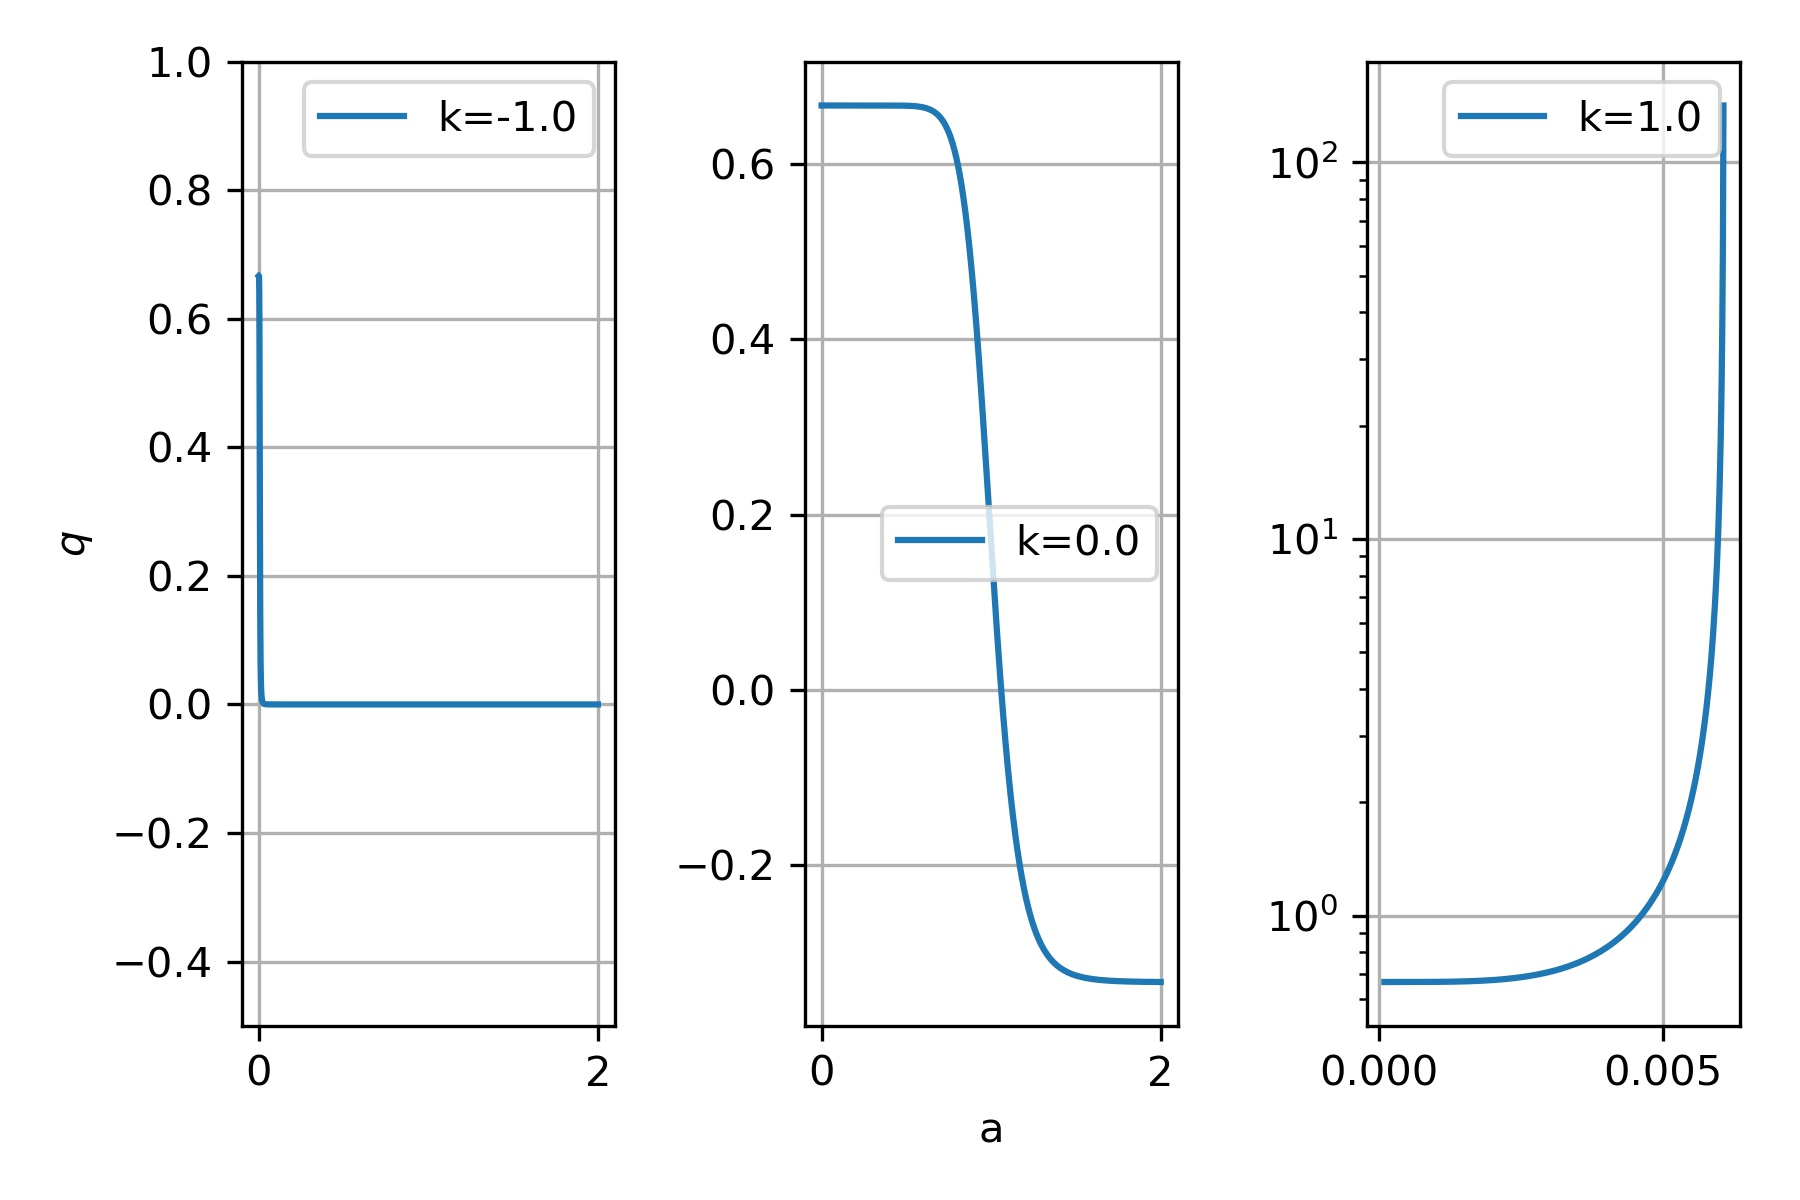
\includegraphics[scale=0.8]{Figures/ch_q.jpg}
\caption{The deceleration parameter for larger red-shifts shows a decelerating expansion, which corresponds to a dust dominated epoch, which changes to a accelerating expansion for small red-shifts, which corresponds to a dark energy dominated epoch.}
\renewcommand{\baselinestretch}{0.85}
\label{fig:ChDecel}
\end{figure}
\end{minipage}
%\begin{figure}[H]
%\centering
%\includegraphics[scale=0.9]{Figures/ch_rho.jpg}
%\caption{Here we have taken $A_{1}=50$ and $A_{2}=C_{2}=1$. }
%\label{fig:ChRho}
%\end{figure}


\color{Navy} % Navy color for the abstract
\section*{Solving the Friedman equation for the MCG}
Substituting equation (\ref{eq:ReFMCG}) into the Friedman equation (\ref{eq:CurvFriedman}), assuming a flat curvature and solving the resulting ODE yields:
\begin{equation}\label{eq:FmEqMCGSol}
\begin{split}
\brac{t-t_{0}}&=\frac{2}{3A^{\frac{1}{2}}B_{2}^{\frac{1}{2\beta}}B_{1}}\brac{\frac{B_{3}}{B_{2}}a^{-3B_{1}\beta}+1}^{-\frac{1}{2\beta}}\\
+\\ \frac{1}{2\beta+1}&\brac{\frac{B_{3}}{B_{2}}a^{-3B_{1}\beta}+1}^{-1-\frac{1}{2\beta}}\ _{2}F_{1}\brac{1,1+\frac{1}{2\beta};2+\frac{1}{2\beta};\brac{\frac{B_{3}}{B_{2}}a^{-3B_{1}\beta}+1}^{-1}},\\
\end{split}
\end{equation}
where $_{2}F_{1}\brac{a,b;c;x}$ is the hypergeometric function. \\

\section*{Behaviour of of the deceleration parameter for the case of a Chaplygin equation of state}
Define the deceleration parameter $q\equiv -\frac{\ddot{a}}{a}\brac{\frac{a}{\dot{a}}}^{2}$. Substituting the Raychaudhuri equation (\ref{eq:RayEq}) and Friedmann equation (\ref{eq:CurvFriedman}) for the case of a Chaplygin gas equation of state, in terms of red-shift $z=a^{-1}-1$ into the definition of the deceleration parameter gives:
\begin{equation}\label{eq:ChModDecelZ}
\begin{split}
q &= \frac{\frac{A}{2}\brac{\brac{3B_{1}-2}\brac{B_{3}\brac{1+z}^{3B_{1}\beta}+B_{2}}^{\frac{1}{\beta}}-3B_{1}B_{2}\brac{B_{3}\brac{1+z}^{3\beta B_{1}}+B_{2}}^{\frac{1-\beta}{\beta}}}}{A\brac{B_{3}\brac{1+z}^{3\brac{\beta}\brac{B_{1}}}+B_{2}}^{\frac{1}{\beta}} -\kappa F\brac{1+z}^{2}}.
\end{split}
\end{equation}
The behaviour of equation (\ref{eq:ChModDecelZ}) for all three different curvatures can be seen in figure \ref{fig:ChDecel}. 
%\begin{figure}[H]
%\centering
%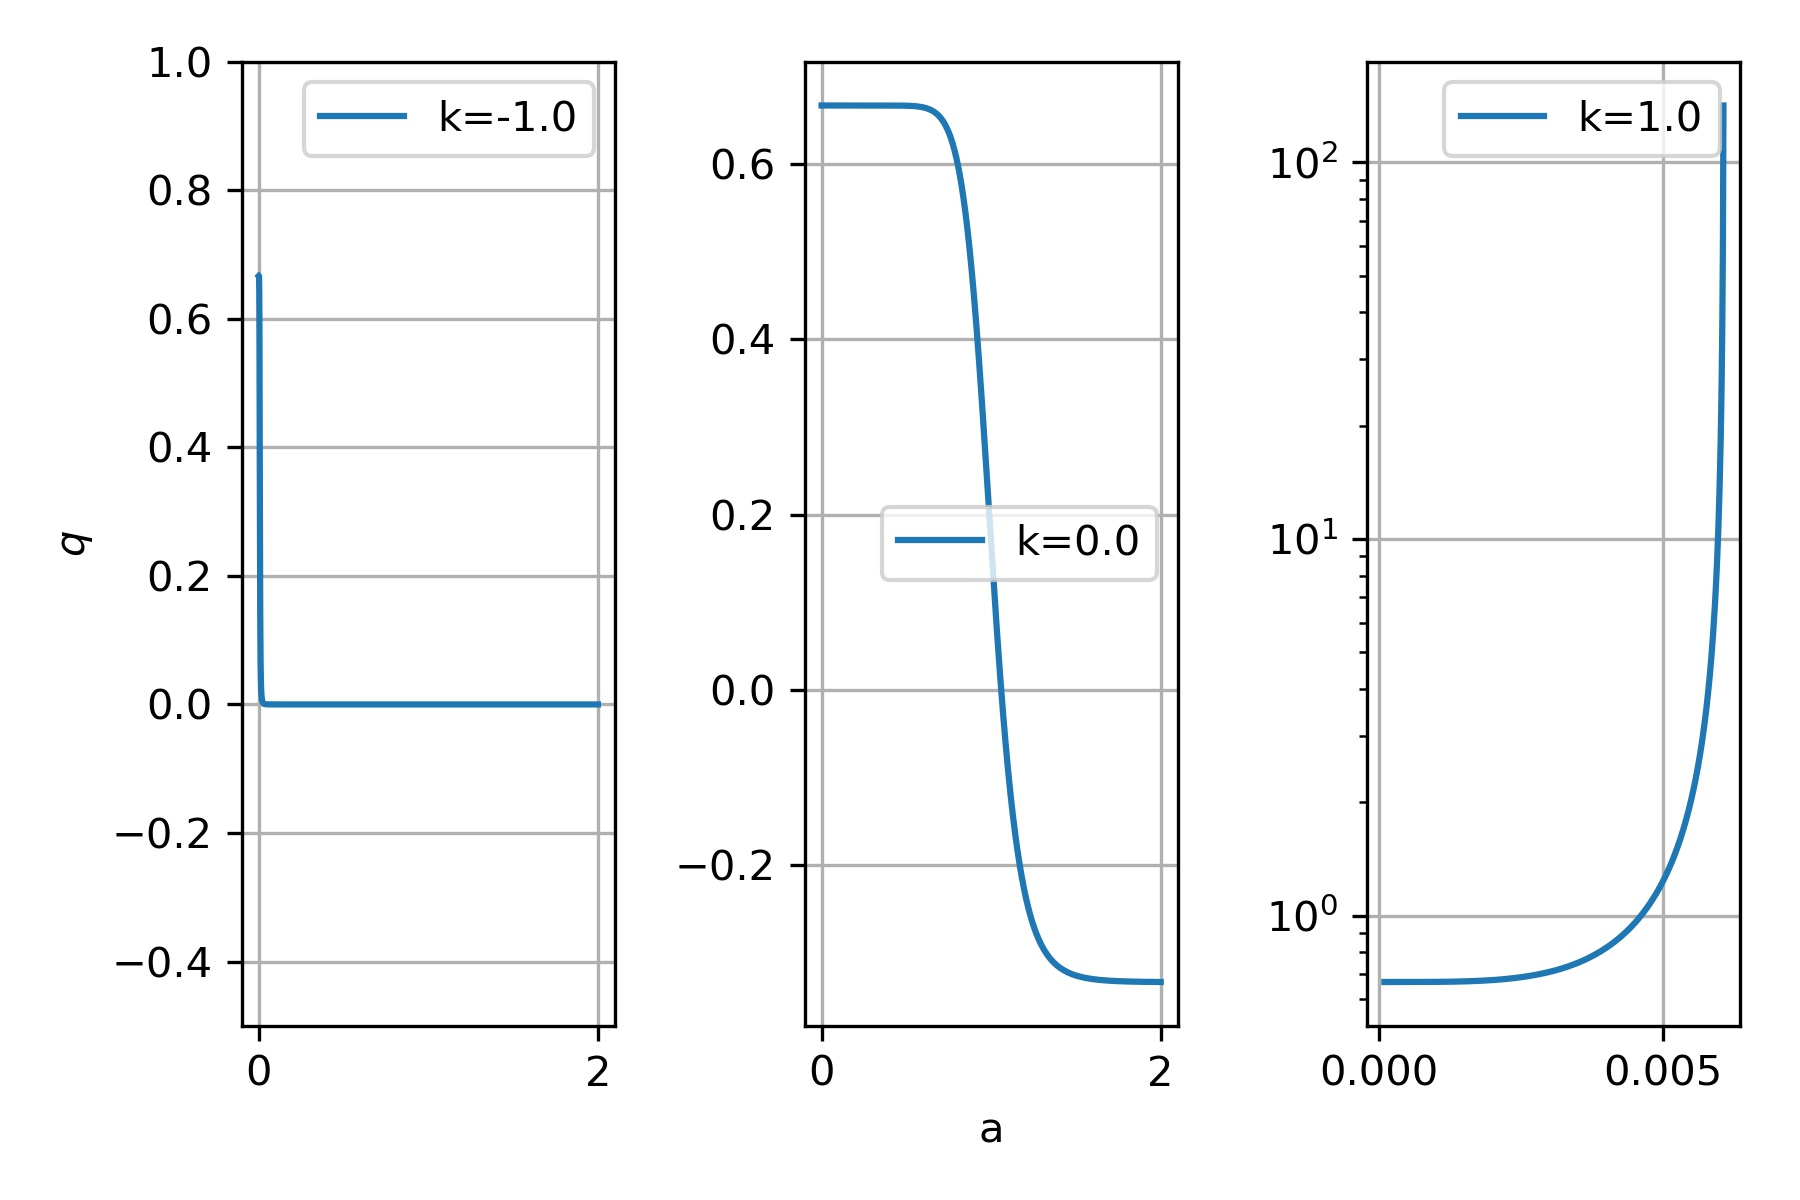
\includegraphics[scale=0.8]{Figures/ch_q.jpg}
%\caption{Here all parameters and constants have again been normalized and taken as in the previous figures.}
%\label{fig:ChDecel}
%\end{figure}
From the figure it can be seen that for small red-shifts the deceleration parameter is negative which corresponds to an accelerated expansion. For large red-shifts, the deceleration parameter is positive corresponding to a decelerating universe. The figure also shows a relatively sharp change from positive to negative for the deceleration parameter.

\color{DarkSlateGray} % DarkSlateGray color for the rest of the content
\section*{Unified dark Fluid}
Another possible candidate for dark energy that also aims to unify dark energy and dark matter into a single dark fluid is proposed by \textit{Wang, Yan and Meng} \citep{wang2017new}. The proposed candidate is a perfect fluid equation of state $P=\omega\rho$ that is parametrized between an equation of state that describes a matter (and here by dark matter) dominated universe, and a dark energy dominated universe. 

\section*{The Pressure-Parametrized Unified dark Fluid equation of state}
The proposed equation of state is given as:
\begin{equation}\label{eq:UDFEoS}
\begin{split}
P &= P_{a}+P_{b}\brac{z+\frac{Z}{1+z}},         \\
\end{split}
\end{equation}
with $P_{a}$ and $P_{b}$ free parameters that are to be constrained by observation.
Substituting equation (\ref{eq:UDFEoS}) into the fluid equation (\ref{eq:4}) and solving the resulting first order differential equation, we find the energy density to be:
\begin{equation}\label{eq:UDFFluidSolZ}
\begin{split}
\rho&= -P_{a}+\frac{3}{4}P_{b}\bracc{\brac{1+z}^{-1}-2\brac{1+z}}+C\brac{1+z}^{3}, \\
\end{split}
\end{equation}
where $C$ is an integration constant. Comparing the found solution to the energy densities found for the Concordance model, it can be seen that the first term in equation (\ref{eq:UDFFluidSolZ}) corresponds to that of a dark energy dominated epoch, while the last term corresponds to that of a dust dominated epoch. Plotting the result, we can see the behaviour of the energy density for the pressure-parametrized unified dark fluid (PPUDF) equation of state.
\noindent
\begin{minipage}{.24\textwidth}
\begin{figure}[H]
\centering
\renewcommand{\baselinestretch}{0.5}
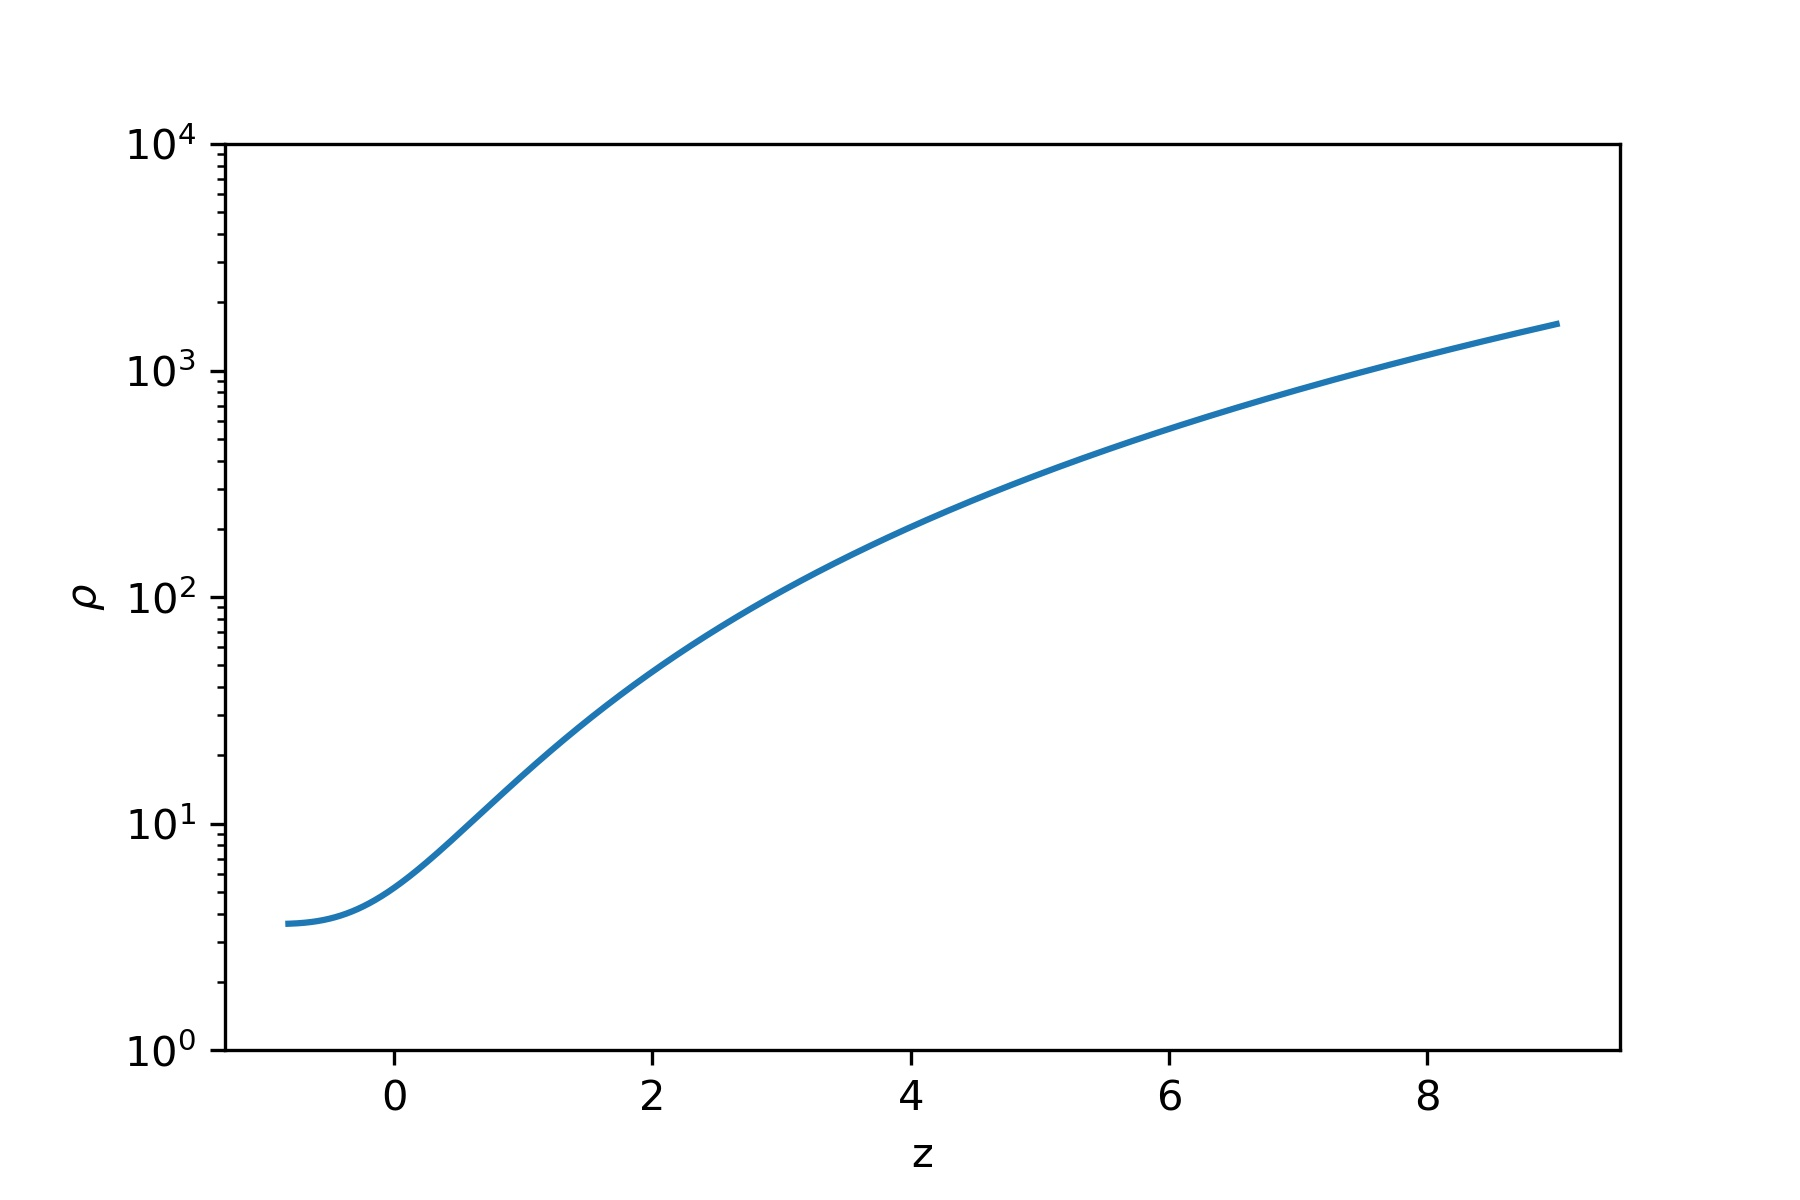
\includegraphics[scale=1]{Figures/UDF_rho.jpg}
\caption{The energy density for a pressure-\\parametrized unified dark fluid equation of state. The\\ energy density is non-linear for larger red-shifts, \\but reduces to approximately constant in the near future.}
\label{fig:UDFRho}
\end{figure}
\end{minipage}% This must go next to `\end{minipage}`
\begin{minipage}{.24\textwidth}
\vspace{20pt}
\begin{figure}[H]
\centering
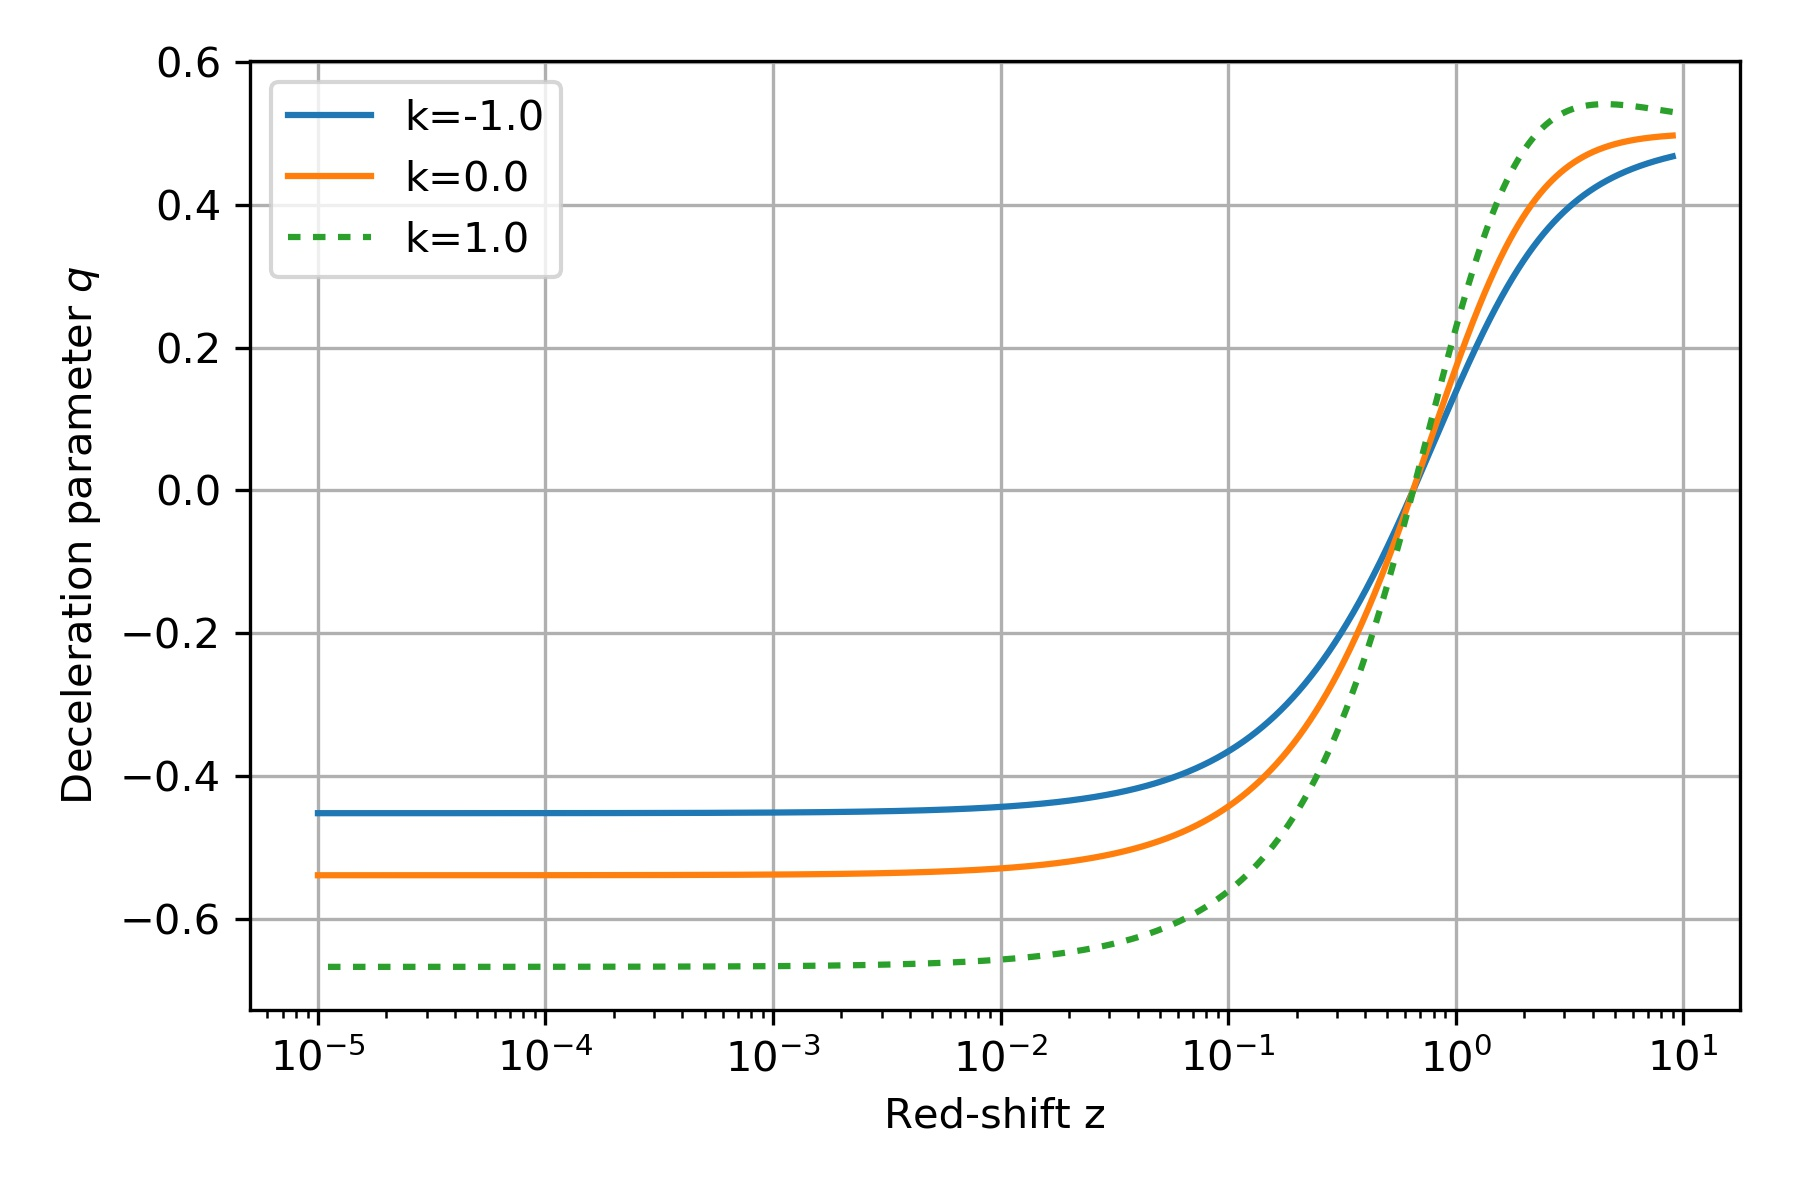
\includegraphics[scale=0.9]{Figures/UDF_q.jpg}
\caption{The behaviour of the deceleration parameter for the case of the PPUDF shows a decelerating expansion for larger red-shifts, which transitions into a accelerating expansion for red-shifts close to zero which is in agreement with an initial dust dominated epoch which transitions into a dark energy dominated epoch. }
\renewcommand{\baselinestretch}{0.85}
\label{fig:UDFq}
\end{figure}
\end{minipage}
%\begin{figure}[H]
%\centering
%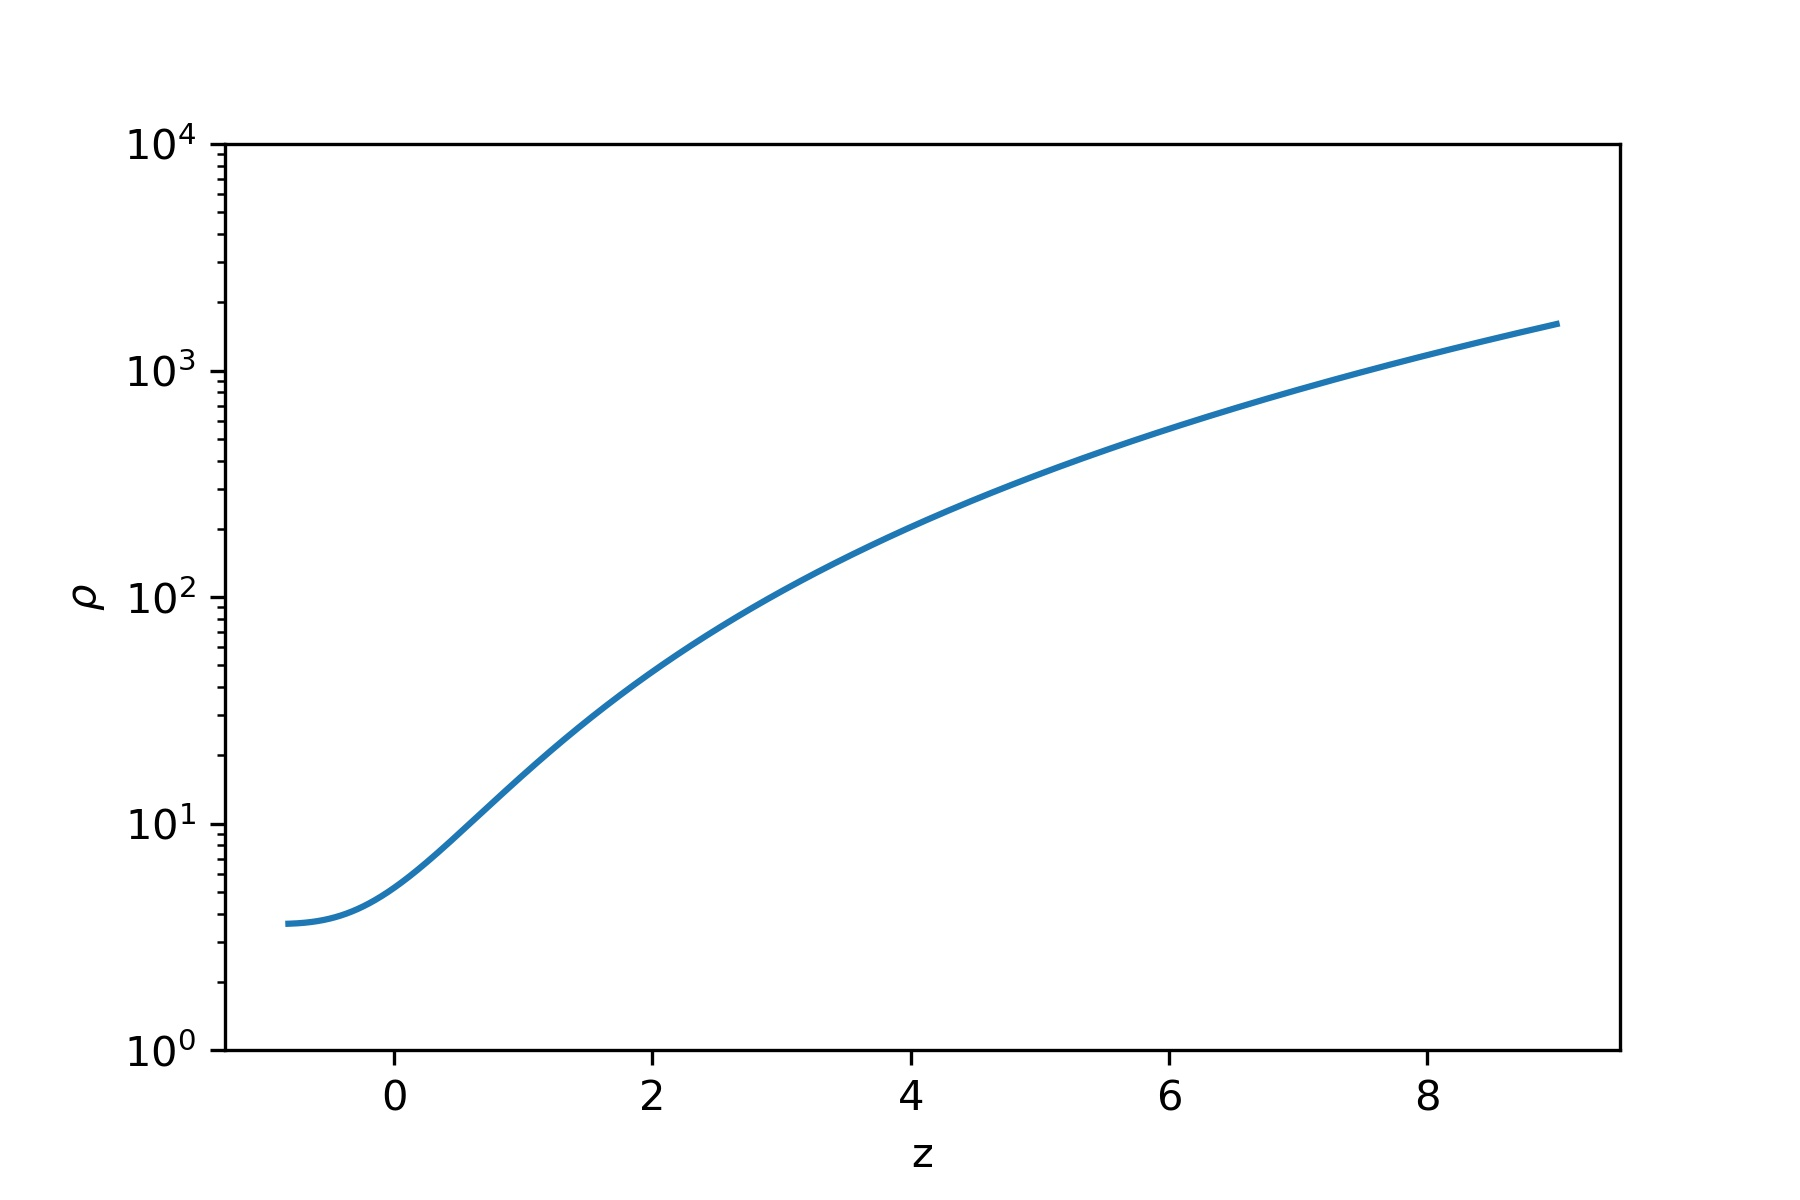
\includegraphics[scale=1]{Figures/UDF_rho.jpg}
%\caption{Here we have arbitrarily taken $P_{a}=-3.6$, $P_{b}=-10^{-5}$ and $C=1.6$.}
%\label{fig:UDFRho}
%\end{figure}
In figure \ref{fig:UDFRho} it can be seen that the energy density increases non-linearly with red-shift, as is expected. It is worth pointing out here that the energy density is sensitive to the values of the free parameters. The plot has also been extended into negative red-shifts to show that the energy density does reduce to an approximately constant energy density in the near future.
\section*{Deceleration parameter for the case of the PPUDF equation of state}
Taking the same approach to find an expression for the deceleration parameter as in equation (\ref{eq:ChModDecelZ}), we find that the deceleration parameter $q$ for the case of the PPUDF is:
\begin{equation}\label{eq:UDFq}
\begin{split}
q &= \frac{A\bracc{2P_{a}-\frac{3}{2}P_{b}\brac{\frac{3}{2}\brac{1+z}^{-1}+\brac{1+z}}+C\brac{1+z}^{3}}}{2A\brac{-P_{a}+\frac{3}{4}P_{b}\bracc{\brac{1+z}^{-1}-2\brac{1+z}}+C\brac{1+z}^{3}} -\kappa F \brac{1+z}^{2}}.        \\
\end{split}
\end{equation}
It is clear that the deceleration parameter is very sensitive to the values of the free parameters. In figure \ref{fig:UDFq} we again plot the resulting expression for the deceleration parameter as a function of red-shift in order to see the behaviour of the deceleration parameter.
%\begin{figure}[H]
%\centering
%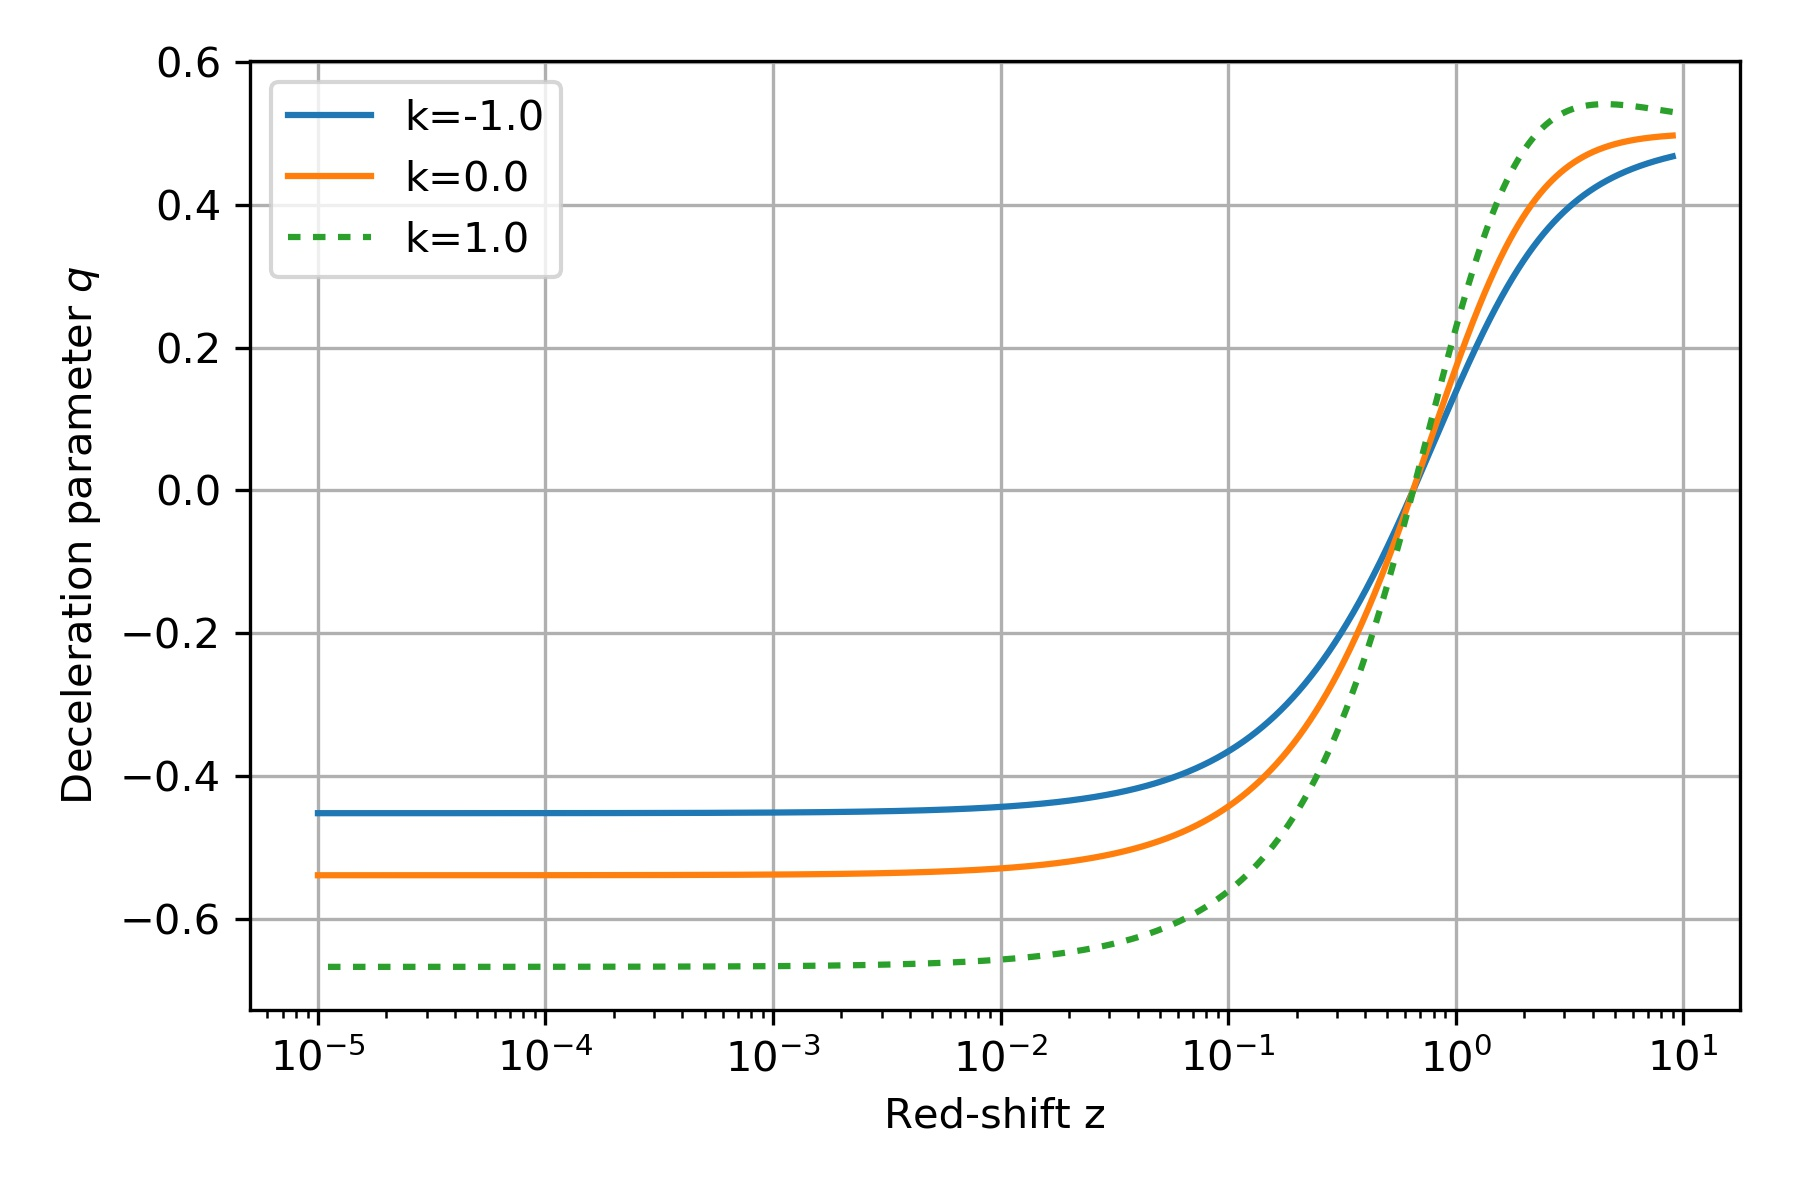
\includegraphics[scale=1]{Figures/UDF_q.jpg}
%\caption{Here the free parameters and constants have been taken to be the same as for the previous figures.}
%\label{fig:UDFq}
%\end{figure}
It is clear from the figure that the PPUDF equation of state also supports a universe that is initially undergoing an approximately constant deceleration that rapidly changes to an approximately constantly accelerating universe for small reed-shifts.

%----------------------------------------------------------------------------------------
%	CONCLUSIONS
%----------------------------------------------------------------------------------------

\color{SaddleBrown} % SaddleBrown color for the conclusions to make them stand out
\section*{Discussion and Conclusions}
From figures \ref{fig:ChRho} and \ref{fig:UDFRho} it is clear that both the Chaplygin gas and the PPUDF equations of state show behaviour of the energy density that corresponds with that of the concordance model for both the dust and dark energy dominated epochs. Both equations of state result in an expression for energy density that is non-linear for large red-shifts. The expression for energy density that results from the Chaplygin gas equation of state also reduces to a constant for small red-shift. For the energy density expression that results from the PPUDF equation of state, figure \ref{fig:UDFRho} shows that the energy density deviates from the Concordance model for small red-shifts, but reduces to the concordance model in the near future which is consistent with the findings of \textit{Wang, Yan} and \textit{Meng} \citep{wang2017new}. Looking at the behaviour of the dimensionless Hubble parameter that results from using either equation of state, we find that both equations of state are viable when compared to what is expected based on observation. The behaviour of the deceleration parameter that results from both the PPUDF and Chaplygin gas equations of state, support an expansion that is initially decelerating, which then abruptly changes to a near constantly accelerating expansion. The former behaviour is consistent with a dust dominated epoch. The later is consistent with a dark energy dominated epoch. The behaviour resulting from both equations of state are very sensitive to the chosen values of the free parameters and must therefore be constrained by observation.\\
From the resulting behaviour found for both the PPUDF and Chaplygin gas equations of state, it is clear that it is possible to parametrize the equations of state for the dust dominated epoch and dark energy dominated epoch into that of a single unified dark fluid equation of state that is consistent with the Concordance model.



\color{DarkSlateGray} % Set the color back to DarkSlateGray for the rest of the content

%----------------------------------------------------------------------------------------
%	FORTHCOMING RESEARCH
%----------------------------------------------------------------------------------------



 %----------------------------------------------------------------------------------------
%	REFERENCES
%----------------------------------------------------------------------------------------

%\nocite{*} % Print all references regardless of whether they were cited in the poster or not
\bibliographystyle{unsrt} % Plain referencing style
\bibliography{./References/References} % Use the example bibliography file sample.bib

%%----------------------------------------------------------------------------------------
%%	ACKNOWLEDGEMENTS
%%----------------------------------------------------------------------------------------
\section*{Acknowledgements}
I wish to thank The National Astrophysics and Space Science (NASSP) and  Center for Space Research (CSR) for funding and support as well as Dr. Amare Abebe  and Dr. Bishop Mongwane for their support with the project.



%----------------------------------------------------------------------------------------

\end{multicols}
\end{document}